\chapter{Methods and Concepts}
\label{sec:fepest:methods}

The fundamental methods applied by PEST during the calibration process are briefly described in the following. As already mentioned in section \ref{sec:fepest:ThisManual}, this description allows the reader to quickly understand their respective role in the overall workflow. The PEST documentation, to which specific references are provided, describes the methods in full detail.

\section{GLMA Search Algorithm}

The central feature of the PEST engine is the GLMA search algorithm, that iteratively optimizes the model parameters to improve its fit to observed data and other objectives. 

The fit to the observations is hereby expressed through the \textbf{Measurement Objective Function}. In the simplest case, this will be the weighted sum of squares of the residuals between measurement and simulation results: 

\begin{equation}
\Phi = \Sigma_i w_i \cdot (h_i^{obs} - h_i^{sim})^2
\label{eq:fepest:objectiveFunction}
\end{equation}

where $(h^{obs}$ denotes an observation (typically from a field measurement), $h^{sim}$ its related simulation result, and $w$ the weight that has been applied to the measurement (observation weights will be discussed in section \ref{sec:fepest:observationWeights}).

The equation \ref{eq:fepest:objectiveFunction} is also the formulation FePEST uses to define the measurement objective function. The observations $h_i$ are loaded from the FEFLOW model and the weights $w_i$ can be changed by the user within the user interface (Figure \ref{fig:fepest:ObservationDefintion}, see also section \ref{sec:fepest:observationDefintion}). 

\begin{figure}
	\center
	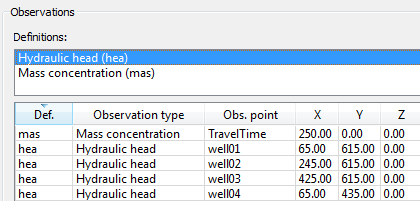
\includegraphics[width=\columnwidth]{figures/ObservationDefintion.png}
\caption{The objective function is defined through the observation definition in FePEST}
\label{fig:fepest:ObservationDefintion}
\end{figure}

The search algorithm used in PEST is the \textbf{Gauss-Levenberg-Marquardt algorithm (GLMA)}. The GLMA changes the model parameters until a minimum objective function value is found. Running PEST, the user will observe two working steps per iteration:
\begin{itemize}
\item Derivative calculation: The parameters are changed incrementally. By repeating the model run for each parameter, and observing the resulting changes of observation values, the partial derivative for each pair of parameter and observation can be calculated by finite-difference approximation. These derivatives form the elements of the \textbf{Jacobian matrix}. The numerical effort to calculate the Jacobian matrix usually dominates the iteration.
\item The parameter values are adjusted in order to reduce the objective function. The direction and magnitude of adjustment is expressed by the \textbf{parameter upgrade vector}. To identify the optimal direction of this vector, the GLMA uses a combination of two strategies:

\begin{itemize}
\item While the objective function shows a predominantly linear behavior, the method of gradient descent is applied. This method determines the parameter upgrade vector by the direction of steepest descent of the objective function. It allows a rapid reduction of the objective function. This can often be observed during the initial phase of the optimization.
\item Objective-function nonlinearity is addressed via the Gauss-Newton method. This method computes a parameter upgrade vector based on the presumption of a quadratic behaviour of the objective function.
\end{itemize}

The two methods are no mutually exclusive: The GLM algorithm interpolates between them, controlled by a scaling parameter (the \textbf{Marquardt-Lambda}). 

PEST dynamically updates lambda depending on the progress in reducing the objective function. The current lambda as displayed by FePEST during the PEST run is a good indicator for the current nonlinearity of the objective function. 

\begin{itemize}
\item high lambda values (e.g., \textgreater 10) indicate linear behavior (and predominant use of the gradient descent method).
\item small values for lambda (e.g., \textless 2) indicate nonlinear behavior (and predominant use of the Gauss-Newton method).
\end{itemize}

Figure \ref{fig:fepest:PhiLambdaCompare} and Figure \ref{fig:fepest:PhiLambdaMap} illustrate the development of the objective function and the Marquardt lambda during a typical PEST optimization. Gradient descent is used in the first iterations, indicated by higher lambda values. When the objective function approaches its (local) minimum, Lambda falls to near zero indicating almost exclusive use of the Gauss-Newton method.

\begin{figure}
	\center
	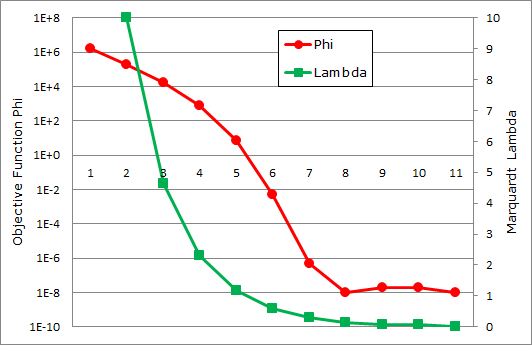
\includegraphics[width=\columnwidth]{figures/PhiLambdaCompare.png}
\caption{Development of the objective function and the Marquardt lambda during a PEST run}
\label{fig:fepest:PhiLambdaCompare}
\end{figure}

\begin{figure}
	\center
	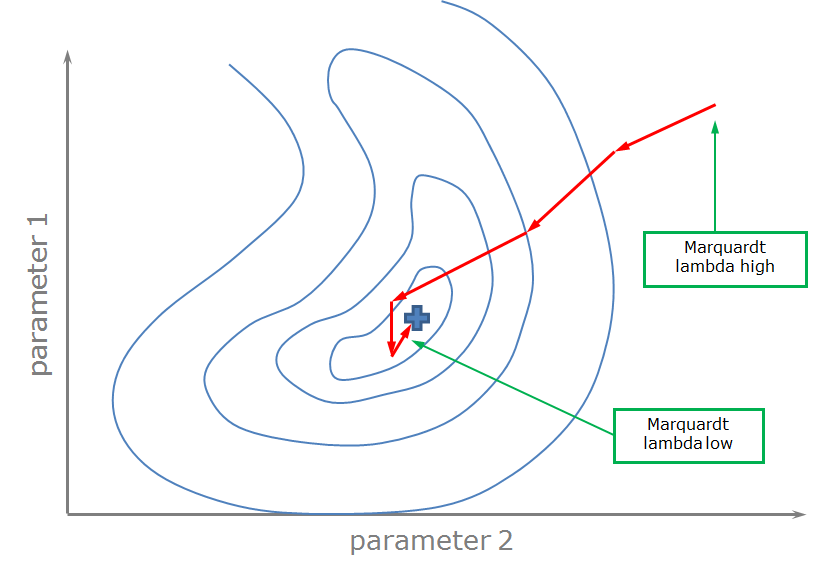
\includegraphics[width=\columnwidth]{figures/PhiLambdaMap.png}
\caption{Schematic illustration of contours of the objective function and the path of the parameter upgrades vectors, after Doherty}
\label{fig:fepest:PhiLambdaMap}
\end{figure}

\end{itemize}

If successful, the GLMA will find a parameter set that constitutes a \textbf{local minimum} of the defined objective function. This is an important restriction because multiple local minima might be present, and it is not guaranteed that the one found is also the global minimum. 

It is therefore possible that different PEST runs result in different parameter sets if the iteration starts at different initial parameter values. These should therefore be chosen as close as possible to those values that are expected.

The modeller should also critically review the resulting parameter set and the model-to-measurement-misfit (see Figure \ref{fig:fepest:FitToData}). Strong, but also very low (see section \ref{sec:fepest:Overfitting}) departures indicate potential problems with the optimization.

\textit{Further reading: PEST Manual (5th Ed.), Ch. 2.1: The Mathematics of PEST.}


\begin{figure}
	\center
	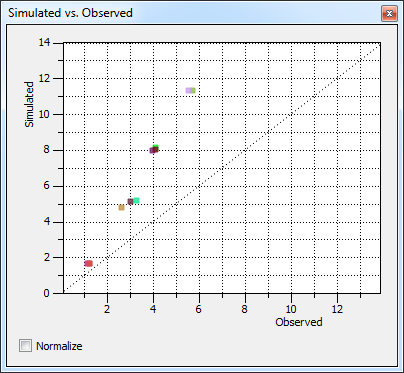
\includegraphics[width=0.7\columnwidth]{figures/FitToDataBefore.png}
	\vspace{0.5cm}\\
	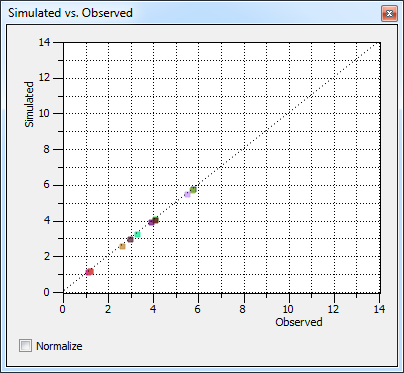
\includegraphics[width=0.7\columnwidth]{figures/FitToDataAfter.png}
\caption{Scatter plot of simulated vs. observed data before (top) and after (bottom) optimization}
\label{fig:fepest:FitToData}
\end{figure}

\subsection{Derivative Calculation}
\label{sec:fepest:derivativeCalculation}

The calculation of derivatives is a fundamental element of the GLM algorithm.

The derivatives are calculated through numerical differentiation. Each parameter is incrementally changed, and the model is run each time to calculate and record the resulting change of the model observations. The derivative of each parameter – observation relationship is then calculated through finite-difference techniques.

Correct calculation of derivatives is of critical importance to the optimization, as failure to it will lead to an unstable optimization procedure and PEST will not be able to lower the objective function.

\textbf{Model instabilities} are a frequent cause of PEST failures!

Instabilities introduce noise to the observation, which is random and not related to the physical-based simulation result. Figure \ref{fig:fepest:ModelGranularity} illustrates this effect. If this noise - and not the incremental parameter change - dominates the observation response, the direction of the parameter upgrade vector becomes random itself and the optimization will fail.

\begin{figure}
	\center
	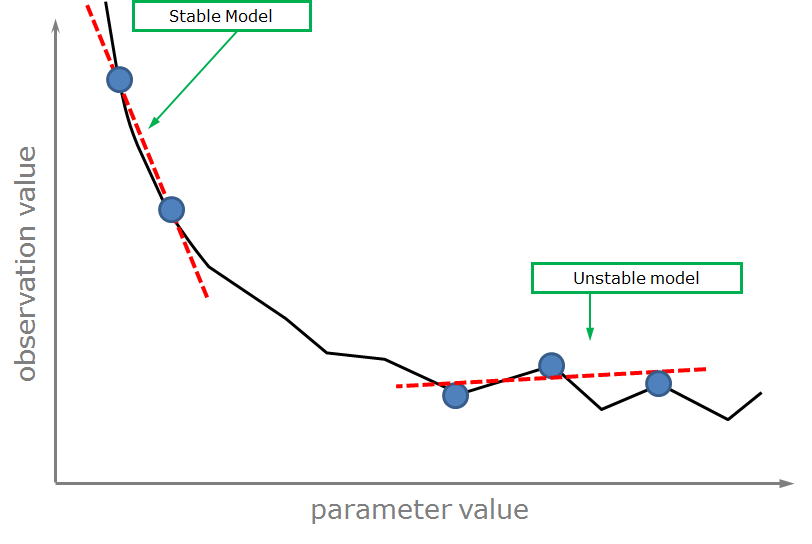
\includegraphics[width=\columnwidth]{figures/ModelGranularity.png}
\caption{Calculation of derivatives during stable (left) and unstable (right) model behavior. If the model is unstable, random noise dominates the physical-based change of the observation value. PEST tries to compensate with higher order finite-difference methods.}
\label{fig:fepest:ModelGranularity}
\end{figure}

Even though certain countermeasures are available (see section \ref{sec:fepest:parameterGroupsSettings}), the modeller should always aim at maintaining maximum stability of the FEFLOW model. With \textbf{JACTEST} (section \ref{sec:fepest:Jactest}), PEST provides a tool to check the integrity of the derivatives calculation for specified parameters. 

%However, the choice of a larger increment size (risk of leaving the quasi-linear parameter increment) or using three- or five-point calculation points (significant increase of required model calls) should be used as a last resort only. The respective settings are described in section \ref{xyz}.

\textit{Further reading: PEST Manual (5th Ed.), Ch. 2.3: The Calculation of Derivatives.}

\subsection{Observation Weights}
\label{sec:fepest:observationWeights}

The weight of an observation controls how strong its residual (the deviation between computed and measured result) contributes to the measurement objective function. A reasonable choice of weights can positively influence the convergence behavior and result of the GLM algorithm.  

Different weighting strategies can be applied (alone or in combination), some examples are given in the following.


\begin{itemize}
%\item TODO: Weight by Experience

\item Weighting by Measurement Noise

A common strategy of adjusting observation weights is applying the inverse of its expected measurement noise as a weight factor. The contribution of less trustworthy observation values to the measurement objective function is reduced, limiting the risk of inaccurate measurements having a negative impact on the optimization and leading to the estimation of parameter values which are thereby in error.

\item Weighting by Absolute Measurement Value

The absolute values of observations in a PEST optimization can encompass several orders of magnitudes, especially (but not limited to) if observations of different types are involved (e.g., Hydraulic head [m] and Mass-concentrations [mg/l]).

Observations with small values are therefore under-represented in the measurement objective function. Normalizing the values by assigning a weight equal to the inverse of the absolute compensates for this effect and makes sure that the information contained in these values finds appropriate representation in the optimization.

\item Equalizing Observation Group Contributions
 
Observations of different types are assigned to different observation groups. One may also decide to manually assign observations of the same type to different observation groups. Using a spreadsheet or the PEST tool PWTADJ1 observation weights can be adjusted to equalize the total contribution of each observation group to the total objective function at the start of the optimization process. This helps to ensure that the information that is contained in each of these observation groups is used in estimation of model parameters, and not undervalued or overvalued because of too low or too high a contribution to the initial objective function.

\item Declustering
 
Observations can be correlated. Water level measurements at observation wells close to each other are often not independent. It is likely that values and changes at these wells are similar, and the worth of information contributed by one well is diminished because it was already contributed by a different well in its vicinity. The worth of information provided by each well is therefore lower than a separate measurement at a larger distance. In this case, the weight of correlated observations should be reduced.

\item Sampling Frequency (Time series)

Weighting by sampling frequency can be seen as a special case of declustering. Observations in time series are often correlated as well. Daily measurements of the groundwater level might carry the same worth of information as a measurement taken on a monthly basis does. Because the daily measurement has more measurement points, it would be overrepresented if the weights of each measurement point is not compensated for. This makes it advisable to normalize the weights of observations of time series by the sampling rate of the measurement.

Weighting by inverse sampling rate is a first-order correction of time-series type observations. The weights are chosen proportionally to the time period that relates to each sample sample, see Figure \ref{fig:fepest:TSweighting}.

\begin{figure}
	\center
	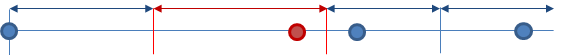
\includegraphics[width=\columnwidth]{figures/TSweighting.png}
\caption{Calculating weights to correct for different sampling rates across different or within the same time series. The weight is calculated as the half of the time span between neighbouring data samples.}
\label{fig:fepest:TSweighting}
\end{figure}

\end{itemize}

\textit{Further reading: PEST Manual (5th Ed.), Ch. 2.1.2: Observation Weights.}

\section{Pilot-Point Method}

The pilot-point method defines parameters as a spatially variable distribution.

In the classical calibration approach, it is a common assumption that geologic formations have spatially constant parameter values. In reality, this is rarely true.

Therefore, instead of applying a homogeneous parameter value across a zone, varying values for the parameter are assigned at particular locations (the \textbf{pilot points}). Each pilot point represents an adjustable parameter in PEST. An interpolation method then creates a continuous distribution of this parameter. Figure \ref{fig:fepest:PilotPointInterpolation} illustrates the method.

The resulting large number of parameters adds to the degrees of freedom in the inversion process. This will generally lead to a better fit to the measurement data. At the same time, it will increase the level of non-uniqueness and therefore better reproduce the uncertainty associated with the model predictions.


\begin{figure}
	\center
	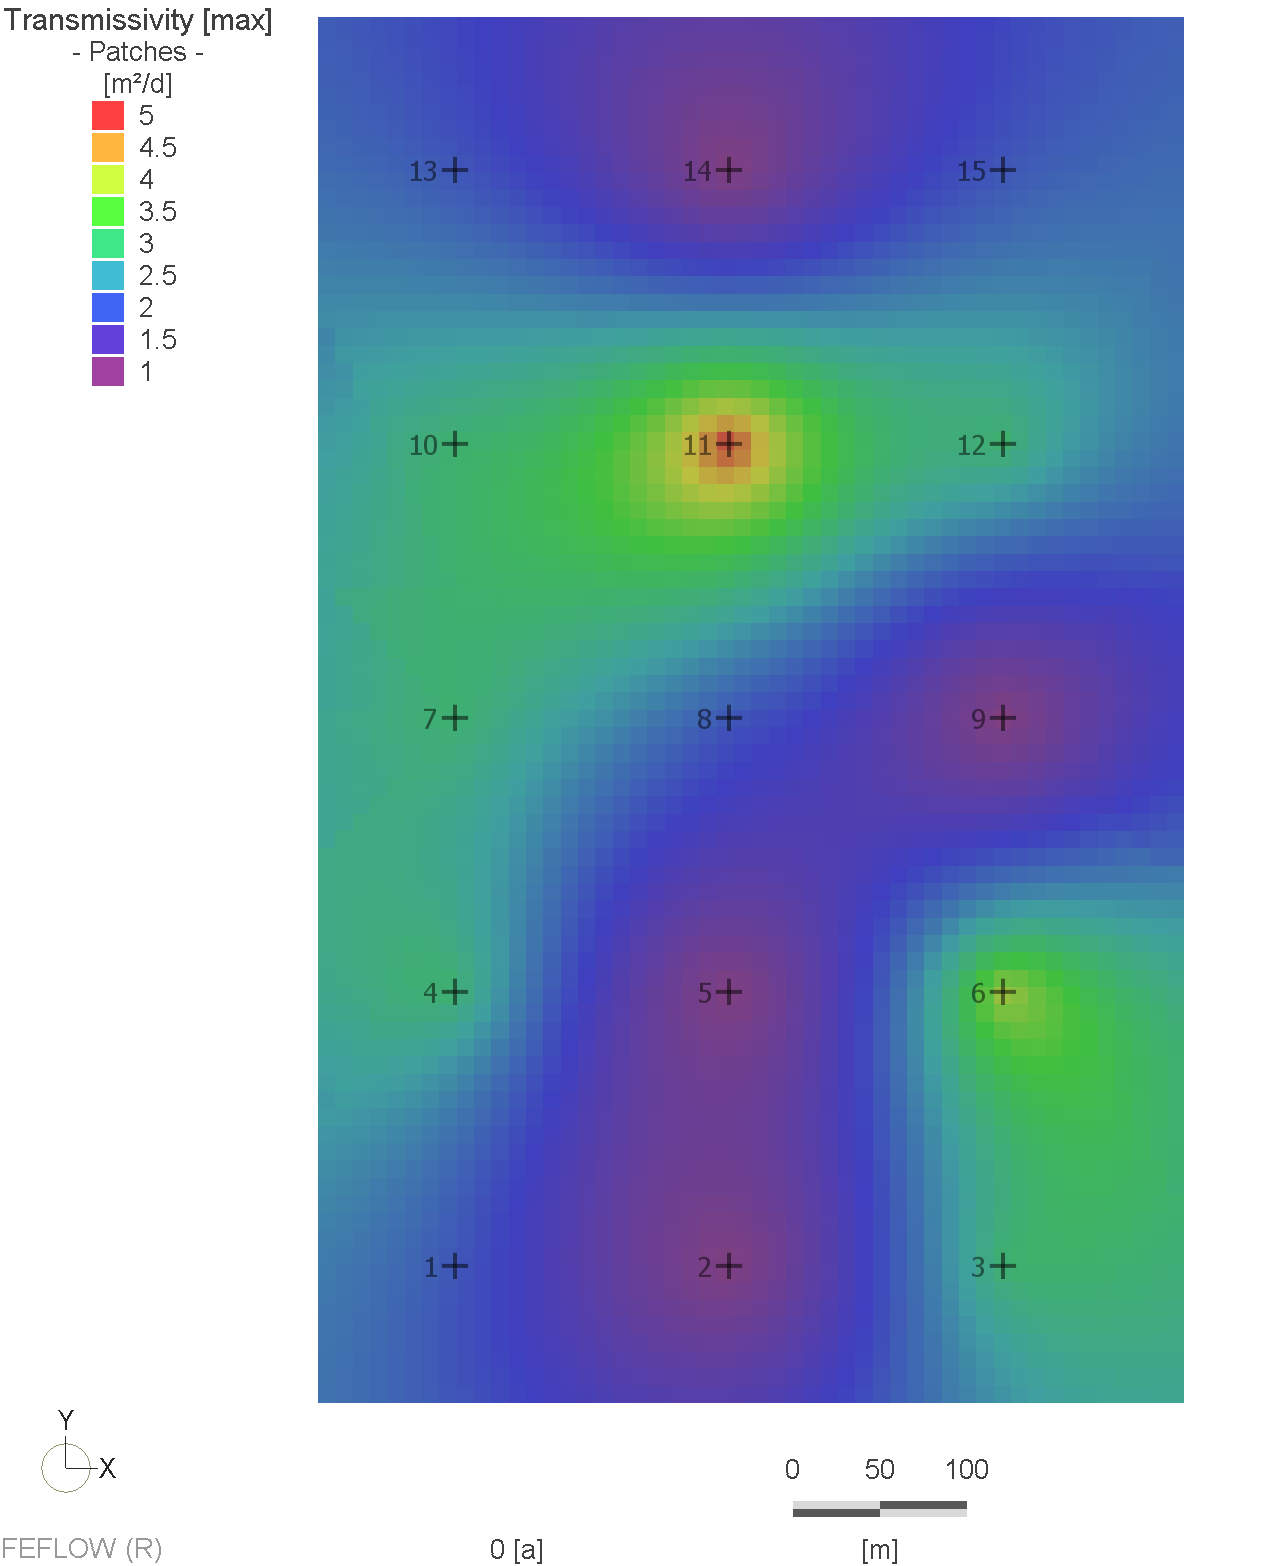
\includegraphics[width=\columnwidth]{figures/PilotPointInterpolation.png}
\caption{Distribution of hydraulic transmissivity, interpolated from a set of 15 pilot points.}
\label{fig:fepest:PilotPointInterpolation}
\end{figure}

Pilot-points often lead to lower objective functions and better fits to measured data. However, the modeller should be aware of the risk of \textbf{overfitting} the parameter field and should always check that the solution is plausible in a geological sense, and regularize it if necessary (see section \ref{sec:fepest:Tikhonov}).

\textit{Further reading: PEST Groundwater Data Utilities, Part A, ch. 5: Model Parameterisation based on pilot-points.}

\section{Parameter Non-Uniqueness}

A typical challenge when history-matching (calibrating) an environmental model is the inherent \textbf{nonuniqueness} associated to the inverse solution. Usually many different parameter sets exist which are all compatible with the historical observation data.

Observation data is usually sparse and usually not sufficient to uniquely identify more than just a few of the large number of model parameters that can be made adjustable.

This has two consequences:

\begin{itemize}
\item Different calibrated parameter sets lead to different predictions. This makes it difficult to use a single model alone for decision-making. 
\item Some or many of the parameters will be insensitive to observations. The GLMA-based optimization process can become unstable under this condition, leading to long optimization run-times or or even failure to optimize.
\end{itemize}

\textbf{Regularization techniques} can provide a defence against these issues. They restrict the parameter search to identifiable parameters, either by adding additional constraints to the parameters (Structural Regularization, \textbf{Tikhonov Regularization}) or separating identifiable parameters from non-identifiable parameters (\textbf{Subspace Regularization}).

This manual restricts itself to Tikhonov regularization (discussed in section \ref{sec:fepest:Tikhonov}) and Subspace regularization (discussed in section \ref{sec:fepest:SubSpaceReg}). 

\textit{See the PEST tutorial} Methodologies and Software for PEST-Based Model Predictive Uncertainty Analysis\textit{, pp. 46 (see the literature review, section \ref{sec:fepest:literatureReview}), for a very good discussion on different regularization techniques.}

\section{Prior Knowledge}
\label{sec:fepest:priorKnowledge}

Prior knowledge is introduced in the optimization if some knowledge about the estimated range of parameters values exists. (This is also referred to as pre-calibration parameter probability.)

The general procedure can be explained in comparison to the history matching process: In history matching, the departure of computed observations from their measured values is expressed as a function (the \textbf{measurement objective function}). Minimizing this function leads to a parameter set that reproduces the historical measurements, hence a calibrated model is found.

When using prior knowledge, the departure of the applied parameter values from parameter values preferred by the modeler is expressed as a second function (the \textbf{regularization objective function}). This kind of regularization is therefore a method that introduces knowledge about the plausibility of parameter values into the calibration process. This knowledge is often subjective, but nevertheless valuable.

PEST implements two principle methods to perform a concurrent optimization on measurement and regularization objective function: Prior Information and Tikhonov Regularization.

\subsection{Prior Information}

Prior Information is the simplest way to implement preference for parameter values or to preferred relationships between them (e.g., a preferred ratio between horizontal and vertical hydraulic conductivity). The sum of squares of departures from these equations contribute to the regularization objective function. 

Minimization of the total of regularization and measurement objective function leads to a parameter set that reproduces the historical measurements and shows a plausible parameter distribution at the same time.

\textit{Further reading: PEST Groundwater Data Utilities (5th Ed.), ch. 2.1.3: The Use of Prior Information in the Parameter Estimation Process.}

\subsection{Tikhonov Regularization}
\label{sec:fepest:Tikhonov}

The Tikhonov regularization method as implemented in PEST automatically generates a number of "prior information" equations, which defines the initial value of each parameter as the preferred value (see Figure \ref{fig:fepest:PrefferedValuesPI}). The user can also make changes to these equation, or setup his/her own additional equations.

\begin{figure}
	\center
	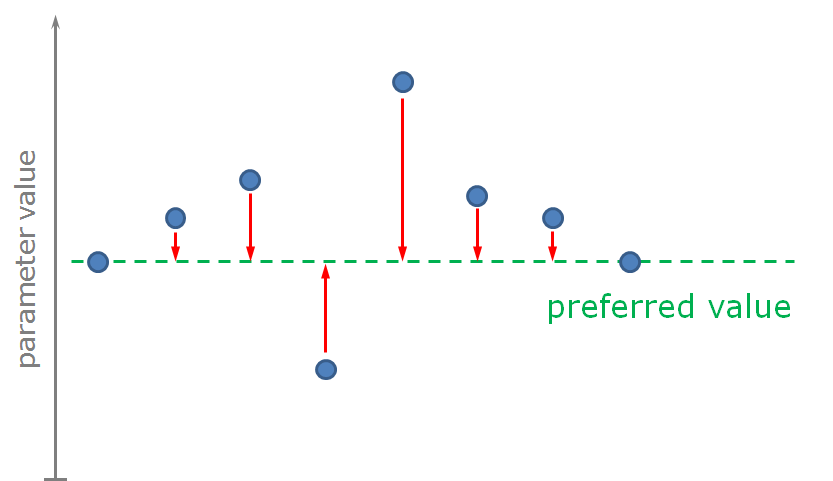
\includegraphics[width=\columnwidth]{figures/PrefferedValuesPI.png}
\caption{Regularization of parameters: departures (red) from preferred parameter values (green) are penalized. The departures contribute to a regularization objective function.}
\label{fig:fepest:PrefferedValuesPI}
\end{figure}

When using Tikhonov regularization the calibration process is formulated as a constrained minimization process as follows “minimize the regularization objective function while ensuring that the measurement objective function is set at the user-specified target”. Figure \ref{fig:fepest:constraintOptimization} illustrates this approach. If this user-specified target is not met, then PEST minimizes the measurement objective function. In the meantime it adjusts weights applied to prior information such that they act as Lagrange multipliers in the constrained optimization process. PEST thus determines the appropriate relative weighting between measurements and respect for prior information in accordance with a user’s choice of target measurement objective function.

\begin{figure}
	\center
	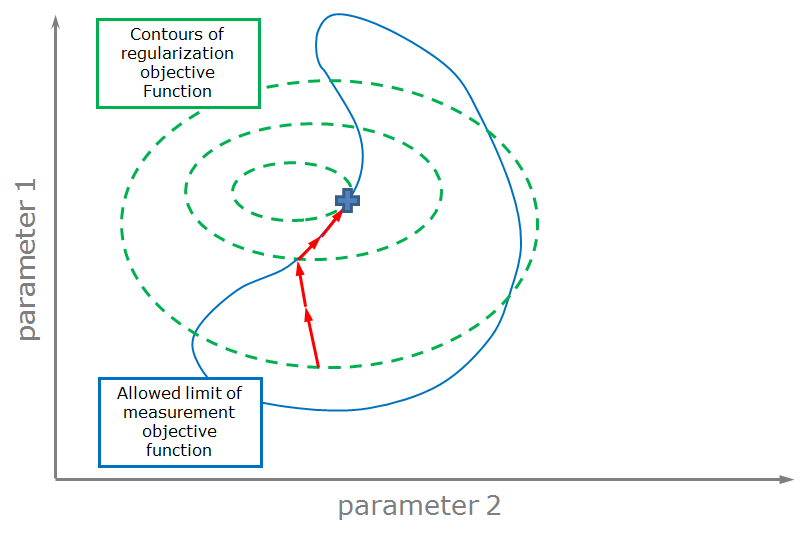
\includegraphics[width=\columnwidth]{figures/constraintOptimization.png}
\caption{Constraint optimization: the regularization objective function (green contours) is minimized while staying within the defined limits (red contour) of the measurement objective function.}
\label{fig:fepest:constraintOptimization}
\end{figure}

As a result, Tikhonov-Regularization reduces the number of possible parameter sets that constitute a calibrated model by rejecting calibrated models with unrealistic parameter values.

Figure \ref{fig:fepest:exampleConstraintOptimization} shows the typical evolution of this process. The model is calibrated using a set of parameters of two different types (hydr. conductivity and recharge). Because the initial parameter values are equal to the preferred values (the prior knowledge) the regularization objectives are initially zero.

\begin{figure}
	\center
	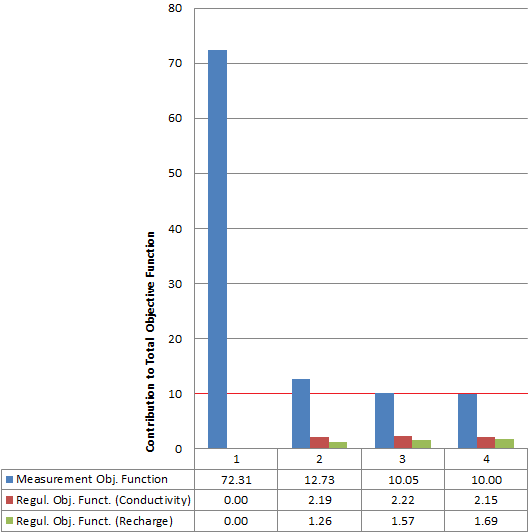
\includegraphics[width=\columnwidth]{figures/exampleConstraintOptimization.png}
\caption{Behaviour of different objectives during constrained optimization. Regularization objectives are kept to a minimum while the observation objective is reduced to its target value PHIMLIM = 10 (red line).}
\label{fig:fepest:exampleConstraintOptimization}
\end{figure}

In order to calibrate the model and reduce the measurement objective, departures from these preferred values are necessary, giving rise to the respective regularization objective. The regularization objectives are however kept to a minimum during the process, keeping the parameters values as close to the preference as possible.

As opposed to classical calibration, the measurement objective is  not minimized. It is reduced only to or below a certain target (PHIMLIM). This  is related to the confidence the modeller has into the measurements that constitute the measurement objective function: The smaller the measurement error is assumed to be, the higher is the necessity to reproduce the observations with the model. 

In this example a limit of PHIMLIM = 10 was used, which has been derived by summing up the weighted confidence intervals of the measurements (10 boreholes, each with a confidence interval of 1~m and a weight of 1).

Further reading: \textit{Methodologies and Software for PEST-Based Model Predictive Uncertainty Analysis: Regularization (p. 46)}


\subsection{Regularization of Pilot Point Parameters}

If parameter fields are defined as a varying distribution using the pilot point method, this will allow a better fit to the observation data during history matching compared to a result obtained using constant parameters. While this is favourable to some extent, the resulting parameter field might look implausible, especially when pilot points are placed at a high density.

\begin{figure}
	\center
	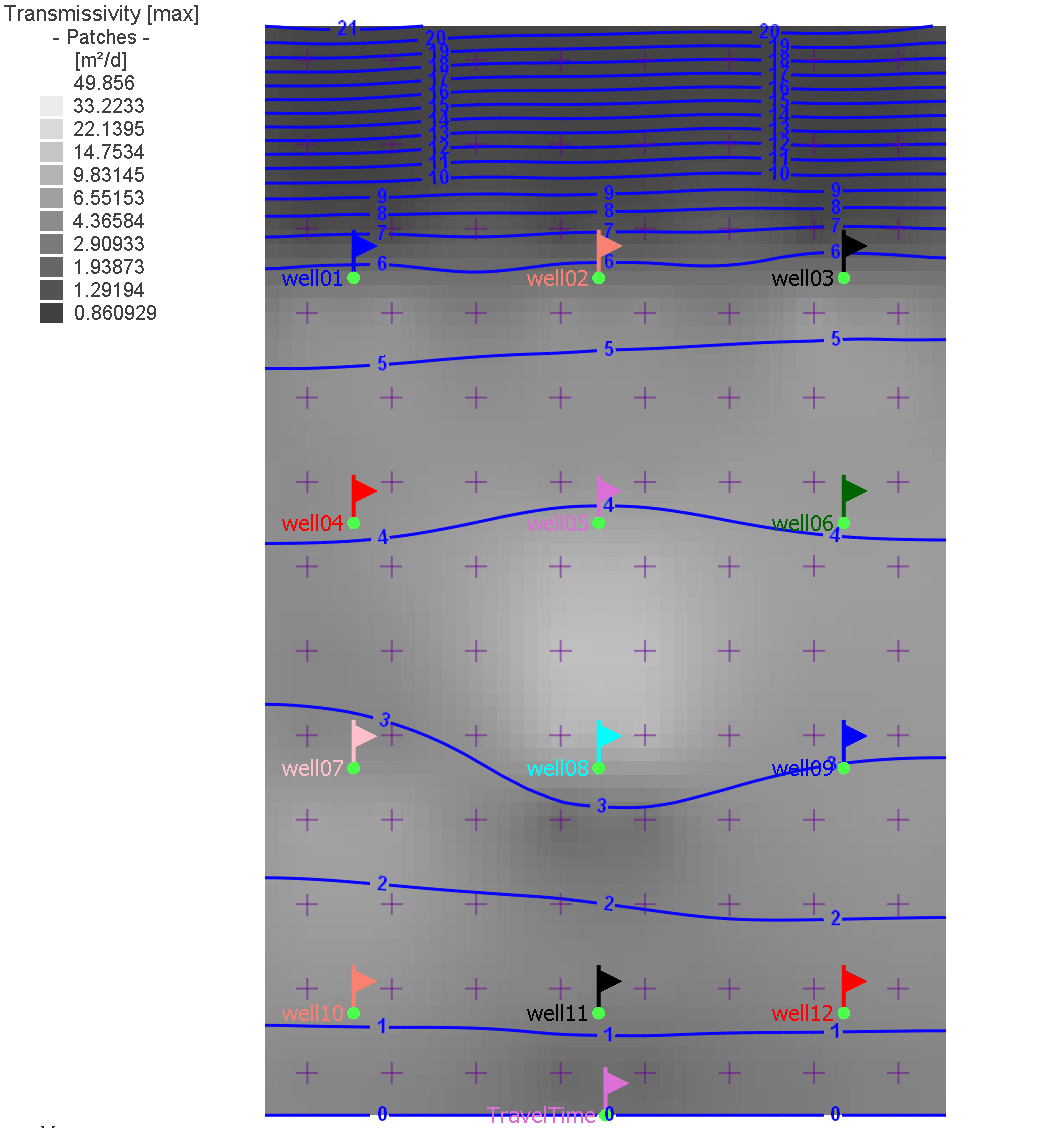
\includegraphics[width=\columnwidth]{figures/CondHeadCalib1.png}
\caption{An overfitted parameter field.}
\label{fig:fepest:CondHeadCalib1}
\end{figure}

Figure \ref{fig:fepest:CondHeadCalib1} provides an example. Because there are more pilot points (104, purple crosses) than observations (12, flags), a perfect match between observed and simulated results is obtained. 

The transmissivity field however reveals that this result is flawed nonetheless: The distribution looks somewhat "bumpy", especially around the observations. Even more severe, the transmissivity above the northernmost row of observation points is totally different (lower) from the one in the remaining area.

A parameter distribution like this is unlikely, and accordingly a prediction made with this model has a high potential of wrongness even though it is perfectly aligned with its calibration data. This state is called \textbf{overfitting}.
\label{sec:fepest:Overfitting}

To prevent overfitting, a second objective (next to the measurement objective function) is required, through that plausibility is preferred.

A common approach is to prefer homogeneous distributions of parameters over heterogeneous distributions. If different values are assigned to neighboring pilot points to lower the measurement objective function, this difference will be penalized and will give rise to the regularization objective function (See figure \ref{fig:fepest:PrefferedValuesSmoothing}). As a consequence, the optimization will yield a balanced compromise between calibration fit and homogeneity.

\begin{figure}
	\center
	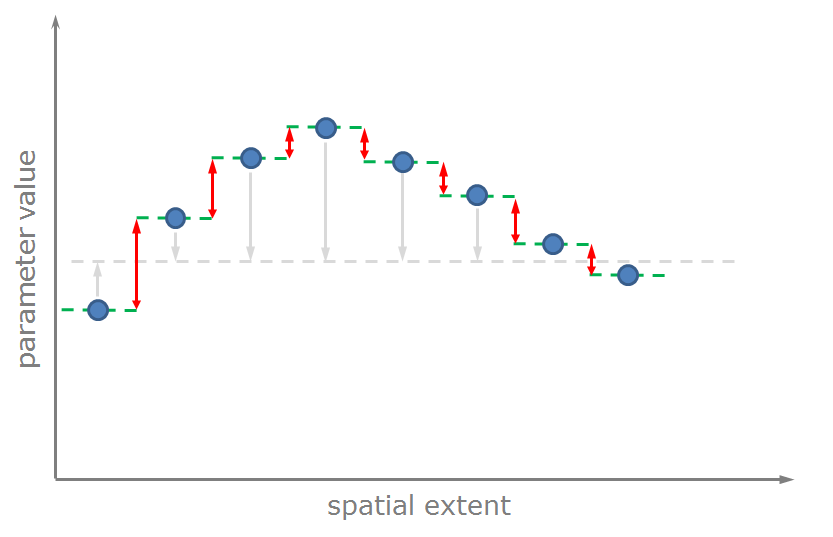
\includegraphics[width=\columnwidth]{figures/PrefferedValuesSmoothing.png}
\caption{Regularization of pilot point parameters: by penalizing differences between pilot points (red), a homogeneous (smooth) distribution is preferred. Initial parameter values are still preferred through prior information (grey).}
\label{fig:fepest:PrefferedValuesSmoothing}
\end{figure}

Finding the right distance within these penalties are applied is important. Differences between closely located points needs to be penalized stronger as the likeliness of parameter differences becomes smaller. Pilot points located far apart (above a certain distance, the \textbf{correlation length}) do not need to be penalized at all. 

This distance and the strength of correlation are defined through a variogram (Figure \ref{fig:fepest:Variogramm200m}). Thus, within the range of correlation, implausible heterogeneities are suppressed unless they are necessary to meet the targeted value of the objective function. PEST calculates the expected correlation between each two pilot points and creates a \textbf{covariance matrix} which is used to impose the correct weights.

\begin{figure}
	\center
	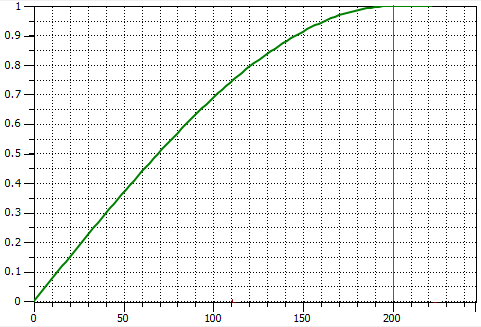
\includegraphics[width=\columnwidth]{figures/Variogramm200m.png}
\caption{A spherical-type variogram with a correlation length (Range) of 200 m.}
\label{fig:fepest:Variogramm200m}
\end{figure}

In summary, the correlation length allows to define a preferred variability of a model property, in addition to the preferred mean value that is provided through the initial parameter value.

Figure \ref{fig:fepest:CondHeadRegularized} shows the same model, regularized with a correlation length of 200~m. The transmissivity field is smoother, but still reflects general trends suggested by the observation data. Even though it yields a stronger model-to-measurement misfit, predictions made using this model will have higher confidence.

\begin{figure}
	\center
 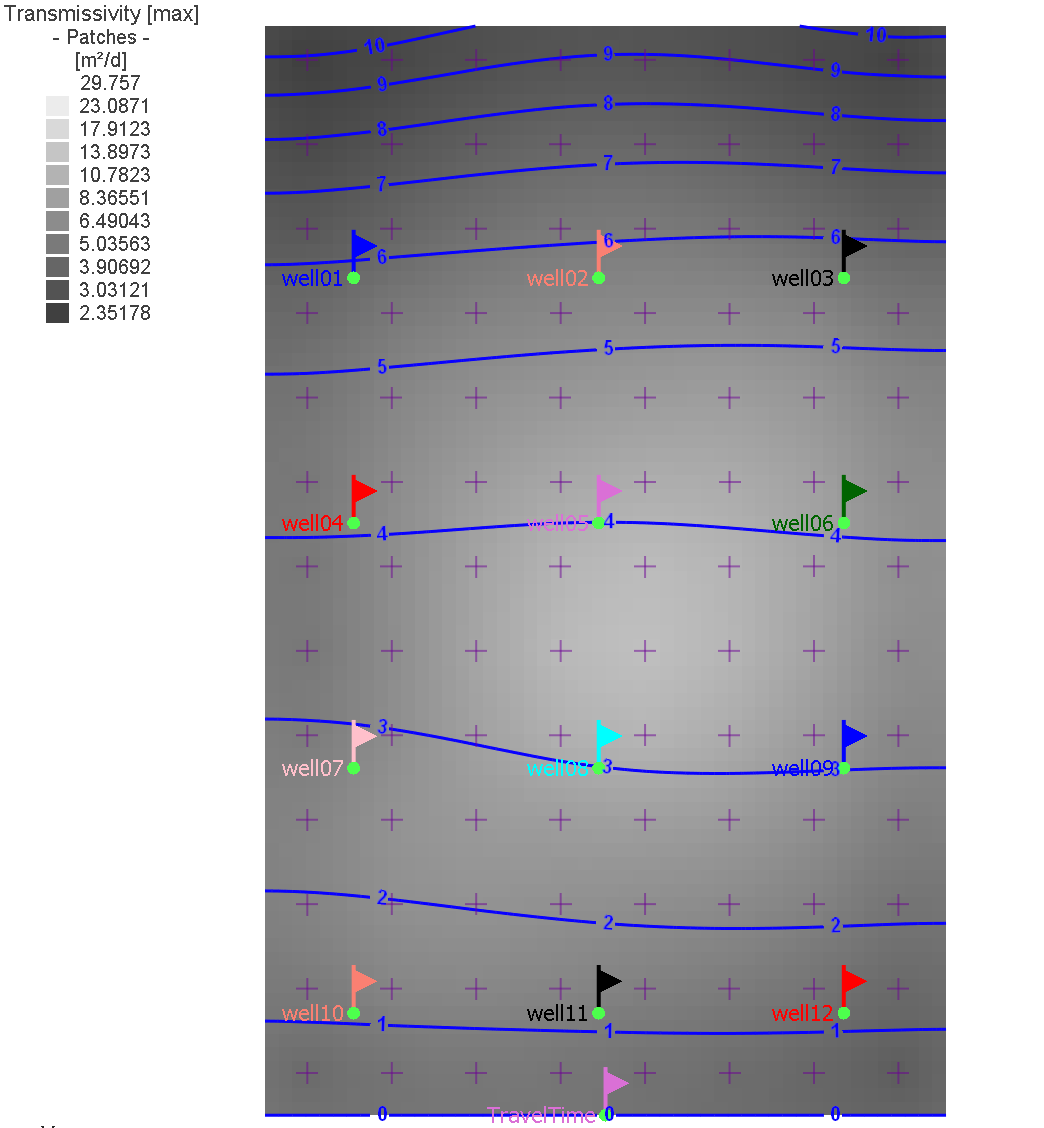
\includegraphics[width=\columnwidth]{figures/CondHeadRegularized.png}
\caption{Regularization of pilot points parameters leads to a smoother parameter field (compare with Figure \ref{fig:fepest:CondHeadCalib1}).}
\label{fig:fepest:CondHeadRegularized}
\end{figure}


\textit{Further reading: PEST Groundwater Data Utilities, ch. 5.6: Regularization (of pilot points)}

%A difference in values of pilot points located within the range of the semi-variogram will be penalized by a rise of the regularization objective function which is greater than if the pilot point parameters are situated further apart. Heterogeneities assumed to be implausible by the expert modeler are therefore suppressed unless they are necessary for achievement of the user-specified target measurement objective function.


%\subsection{Regularization of Pilot Points}

%Fundamentally, a (nearly) homogeneous parameter distribution is usually preferred. That is, neighbouring parameter values are expected to be similar. The distance and strength of the correlation is defined by expert knowledge in the form of a semi-variogram. Thus, within the range of correlation, implausible heterogeneities are suppressed unless they are necessary to meet the targeted value of the objective function.

%\section{Prior Knowledge and Tikhonov Regularization}

%A calibration solution based on the minimization of the objective function alone is non-unique in almost all cases of environmental modelling. Expert knowledge (Prior Knowledge) of the expected geological situations lowers the degree of non-uniqueness by preferring parameter distributions that are considered to be plausible by geological expertise.



\section{Subspace Regularization}
\label{sec:fepest:SubSpaceReg}

Subspace regularization follows a different approach than Tikhonov regularization.

The fundamental idea of subspace regularization is to separate identifiable parameter components from non-identifiable parameter components in order to exclude the latter one from the parameter search. 

The identifiability of a parameter is related to the way and extent it influences existing observation data (if a parameter does not influence any of the existing observations, it cannot be identified).

Parameters (called \textbf{base parameters} in the following) are usually neither completely identifiable or non-identifiable. It is however possible to create linear combinations of base parameters for which this is the case. These are called \textbf{super parameters}.

The transformed (super-)parameter space is separated into two subspaces: One subspace is comprised of combinations of parameters that have an influence on observations. These combinations of parameters can be uniquely estimated through the history matching process.

The remaining parameter combinations occupy the so-called \textbf{null subspace}. These combinations of parameters have no or very small influence on model outputs corresponding to observations; hence estimation of these parameters through history matching is not possible.

The groups are also denoted as sub-spaces of the \textbf{parameter space} (the parameter space is the combination of these two orthogonal subspaces, and contains all parameters):

\begin{itemize}
\item	The group of identifiable parameters is called solution subspace (or often just \textbf{solution space})
\item	The group of non-identifiable parameters is called null subspace (or often just \textbf{null space})
\end{itemize}

\subsection{Truncated Singular Value Decomposition (SVD)}
\textbf{Singular Value Decomposition (SVD)} is the name of the method through which the parameter space is partitioned into the two orthogonal solution and null subspaces.

In most groundwater modeling contexts the solution space is smaller than the null space. The earth is complex, and the information content of most calibration datasets is insufficient to provide unique estimation of the parameters which describe this complexity.

SVD analyzes the \textbf{Eigenvectors} of the the covariance matrix to identify the super parameters. The \textbf{Eigenvalues} - a  measure for the post-calibration variability of their associated Eigenvectors - are the criterion to decide if a parameter is associated with the solution space and therefore included in the optimization or not. 
The ratio of highest to lowest eigenvalue is a measure of the extent to which the inverse problem approaches ill-posedness. If this ratio is more than about 5e-7 then the problem can be considered to be ill-posed (in which case PEST would fail to optimize).

The \textbf{truncated SVD} separates the parameter space into solution and null subspace using this ratio as a criterion, and therefore omits any super parameters that are to insensitive to be uniquely estimated. As a consequence, the inversion of the solution space is always well-posed and a stable optimization is guaranteed (unless flawed by other sources of error, e.g. bad derivative calculation, section \ref{sec:fepest:derivativeCalculation}).

FePEST applies truncated SVD with a threshold of 5e-7 by default in any PEST setup.

\textit{Further reading: PEST Manual (5th Ed.), ch.8.4: Truncated Singular Value Decomposition.}

\subsection{SVD-Assist}

The SVD-A method uses the concept of the SVD to reformulate the inversion problem in a way that it can be solved with much less numerical effort. 

The SVD first identifies those combinations of parameters which are uniquely estimable on the basis of the current calibration dataset and defines them as super parameters. SVD-A creates and run a new PEST setup based on super parameters instead of base parameters. 

When calculating finite-difference derivatives of model outputs with respect to parameters, it actually calculates these derivatives with respect to the super parameters rather than the native model parameters (base parameters). Hence only as many model runs are required per iteration as there are dimensions in the solution space (i.e. number of super parameters).

This method is of fundamental importance for the pilot point method, as it allows calibration and predictive error analysis of highly parametrized models (e.g., using 1000+ parameters) with reasonable effort. 

\textit{Further reading: PEST Manual (5th Ed.), Ch. 8.5 SVD-Assist}

\subsection{Least Squares (LSQR)}

Least Squares (LSQR) is an alternative to the SVD method for highly-parametrized inversion problems. Experience has shown that its application is useful when more than 2500 parameters are involved.

\textit{Further reading: C. C. Paige and M. A. Saunders, LSQR: An algorithm for sparse linear equations and sparse least squares, TOMS 8(1), 43-71 (1982).} and \textit{C. C. Paige and M. A. Saunders, Algorithm 583; LSQR: Sparse linear equations and least-squares problems, TOMS 8(2), 195-209 (1982).}
